\documentclass[10pt,xcolor=pdflatex,hyperref={unicode,hidelinks}]{beamer}

\usepackage{newcent}
\usepackage[utf8]{inputenc}
\usepackage[T1]{fontenc}
\usepackage[czech]{babel}
\usepackage{amsmath,amsfonts,amssymb}
\usepackage{fancyvrb}
\usepackage{url}
\usepackage{algorithmicx}
\usepackage[noend]{algpseudocode}
\usetheme{FIT}

\usepackage{listings}
\usepackage{color}
\lstset{
  language=Go,                    % choose the language of the code
  numbers=left,                   % where to put the line-numbers
  stepnumber=1,                   % the step between two line-numbers.        
  numbersep=5pt,                  % how far the line-numbers are from the code
  backgroundcolor=\color{white},  % choose the background color. You must add \usepackage{color}
  showspaces=false,               % show spaces adding particular underscores
  showstringspaces=false,         % underline spaces within strings
  showtabs=false,                 % show tabs within strings adding particular underscores
  tabsize=4,                      % sets default tabsize
  captionpos=b,                   % sets the caption-position to bottom
  breaklines=true,                % sets automatic line breaking
  breakatwhitespace=true,         % sets if automatic breaks should only happen at whitespace
  %title=\lstname,                % show the filename of files included with \lstinputlisting;
}




\definecolor{dkgreen}{rgb}{0,0.6,0}
\definecolor{gray}{rgb}{0.5,0.5,0.5}
\definecolor{mauve}{rgb}{0.58,0,0.82}




\usepackage{tikz}

\usetikzlibrary{graphs,graphs.standard,arrows.meta,automata,positioning,quotes}

\deftranslation[to=czech]{Definition}{Definice}

\title[IFJ -- projekt: Překladač jazyka IFJ20]{IFJ projekt: Překladač jazyka IFJ20}

\author[]{\textbf{Tým 056, varianta II} \newline František Nečas, Ondřej Ondryáš, David Chocholatý}

\institute[]{Fakulta informačních technologií VUT v Brně\\
Bo\v{z}et\v{e}chova 1/2, 612 00 Brno-Kr\'alovo Pole}

\date{\today}

\begin{document}

\frame[plain]{\titlepage}

\begin{frame}{Rozvržení práce}
    \begin{itemize}
        \item David Chocholatý
            \begin{itemize}
                \item scanner, chybové zprávy na stderr, integrační testy překladače, LL(1)~gramatika, Makefile, hashovací tabulka
            \end{itemize}
        \item František Nečas
            \begin{itemize}
                \item syntaktická analýza (rekurzivní sestup a precedenční SA), základní sémantické kontroly, optimalizace kódu, tvorba vnitřní reprezentace
            \end{itemize}
        \item Ondřej Ondryáš
            \begin{itemize}
                \item datové struktury pro vnitřní reprezentaci kódu (graf řízení toku a abstraktní syntaktický strom), generátor cílového kódu, kostra pro testování, testy pro scanner a parser
            \end{itemize}
    \end{itemize}
\end{frame}

\begin{frame}{Práce v týmu}
    \begin{itemize}
        \item Git (GitHub)
        \item Discord
        \item Virtuální schůzky
        \item Pull request, code review
        \item Párové programování
    \end{itemize}
\end{frame}

\begin{frame}{Návrh překladače}
    \begin{itemize}       
        \item Všechna rozšíření
        \begin{itemize}
            \item BOOLTHEN, BASE, FUNEXP, MULTIVAL, UNARY
        \end{itemize}
        \item Lexikální analyzátor jako konečný automat
        \item Jednoprůchodová syntaktická analýza
        \begin{itemize}
            \item Rekurzivní sestup pro kostru kódu
            \item Precedenční SA pro výrazy včetně přiřazení a volání funkcí
        \end{itemize}
        \item Techniky odloženého odvozování datových typů (suplující druhý průchod SA)
        \item Optimalizace vnitřní reprezentace kódu
        \item Generování kódu – vyhodnocování na zásobníku, zkrácené vyhodnocování logických výrazů
    \end{itemize}
\end{frame}

\begin{frame}{Scanner}
    \begin{itemize}
        \item Deterministický konečný automat
        \item Řešení EOL pravidel
        \item Struktura tokenů
        \item Rozšíření BASE
    \end{itemize}        
    
    \flushright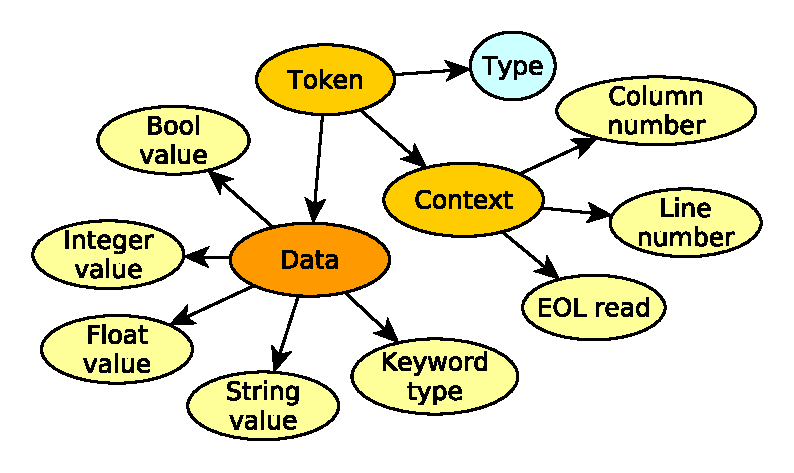
\includegraphics[height=0.6\textheight]{img/pres_token_graph.pdf}

\end{frame}

\begin{frame}{Parser}

    \only<1>{
        \begin{itemize}
            \item Jednoprůchodová syntaktická analýza
            \item Implementace
                \begin{itemize}
                    \item rekurzivní sestup
                    \item precedenční syntaktická analýza
                \end{itemize}
            \item Provádění přidružených sémantických akcí
        \end{itemize}
    }
    \only<2>{
        \begin{itemize}
            \item Zotavení z chyby na základě pevných klíčů (nový řádek)
        \end{itemize}
        \centering\includegraphics[height=0.35\textheight]{img/recover.png}
        \hfill
        \small\flushleft\texttt{parser: error: Line 3, col 15: \\\footnotesize expected float64, int, string or bool keyword, got identifier \\
        \small precedence\_parser: error: Line 4: \\  \footnotesize expected pure expression (no definitions or assignments)}
    }
\end{frame}

\begin{frame}{Precedenční syntaktická analýza}
    \begin{itemize}
        \item Zpracovává výrazy, včetně přiřazení a definicí
        \begin{itemize}
            \item Čárka jako operátor s nejnižší prioritou
            \item Příznak definičních pravidel
        \end{itemize}
        
        \item Detekce konce výrazu (kompatibilní s Go)
        \item Jako sémantické akce vytváří abstraktní syntaktický strom a~provádí typové kontroly
    \end{itemize}
\end{frame}

\begin{frame}{Graf řízení toku}
\begin{columns}[T]
    \column{0.38\textwidth}
        \begin{itemize}
            \item Popis struktury programu
            \begin{itemize}
                \item Lineární + větvení
            \end{itemize}
            \item Metadata programu a funkcí
            \item Čtyři typy vrcholů reprezentujících příkazy
            \item Vrcholy obsahují odkazy na AST
        \end{itemize}
        
        \lstset{xleftmargin=1cm,basicstyle=\small}
        \lstinputlisting{HelloWorld.c}
        
    \column{0.62\textwidth}
        \centering
        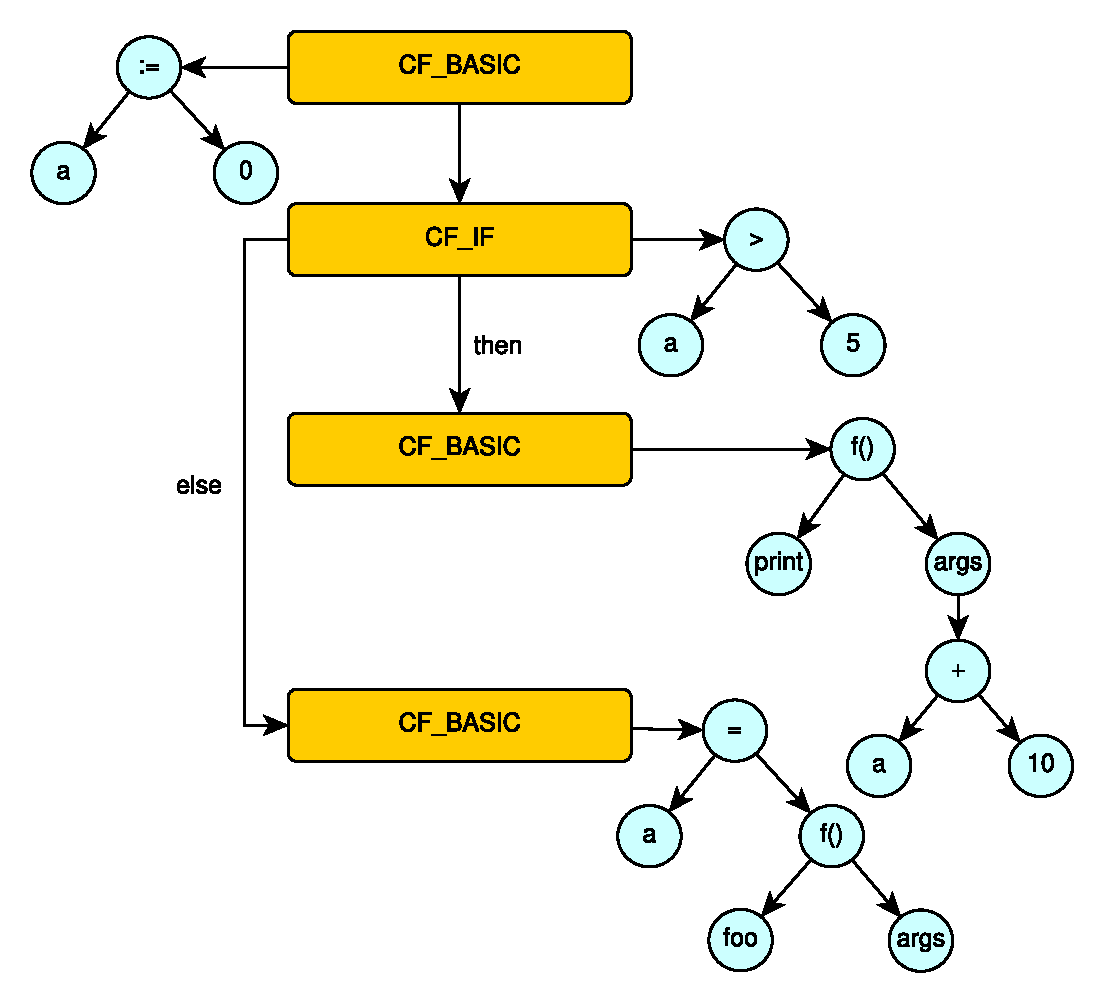
\includegraphics[width=\columnwidth]{img/cfg_ast.pdf}
\end{columns}
    
\end{frame}

\begin{frame}{Abstraktní syntaktický strom}
    \begin{itemize}
        \item Reprezentace výrazu, výstup precedenční SA
        \item Popisuje samotné výpočetní akce
        \item Různé typy uzlů (definice/přiřazení, volání funkcí, operace, termy, \textit{seznam AST})
        \item Zprostředkovává podstatnou část sémantických kontrol -- princip \emph{odvozování datových typů}
        \begin{itemize}
            \item Syntaktický analyzátor při volání funkce ve výrazu ještě nemusel dojít k definici této funkce
            \item Supluje význam druhého průchodu SA
            \begin{itemize}
                \item Zpětně ověřuje správnost volání a typů
            \end{itemize}
        \end{itemize}
    \end{itemize}
\end{frame}

\begin{frame}{Optimalizátor vnitřního kódu}
    \begin{itemize}
        \item Skládání konstant
        \begin{itemize}
            \item Využití algebraických vlastností operací (odstranění dvojité negace)
        \end{itemize}
        \item Propagace konstant
            \begin{itemize}
                \item Sledování konstantních definic v rámci seznamu
                \item Nahrazování proměnných za konstantu
            \end{itemize}
        \item Odstranění mrtvého kódu
        \begin{itemize}
            \item For cyklů s konstantní nepravdivou podmínkou
            \item Else bloků vždy pravdivé podmínky
            \item If bloků se vždy nepravdivou podmínkou
        \end{itemize}
    \end{itemize}
\end{frame}

\begin{frame}{Optimalizátor vnitřního kódu}
    \centering
    \only<1>{
    Původní struktura kódu
    
    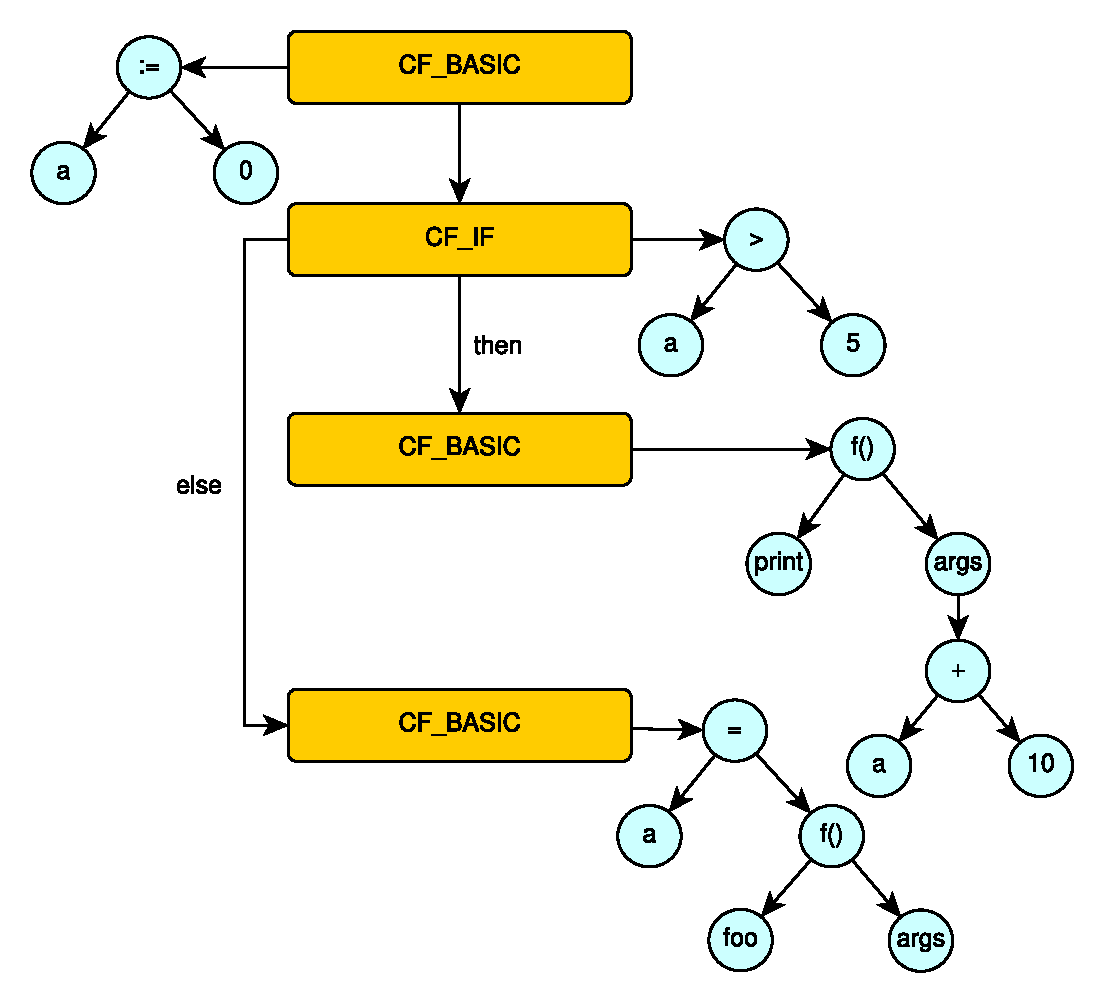
\includegraphics[height=0.8\textheight]{img/cfg_ast.pdf}
    }
    \only<2>{
    Po propagaci konstant
    
    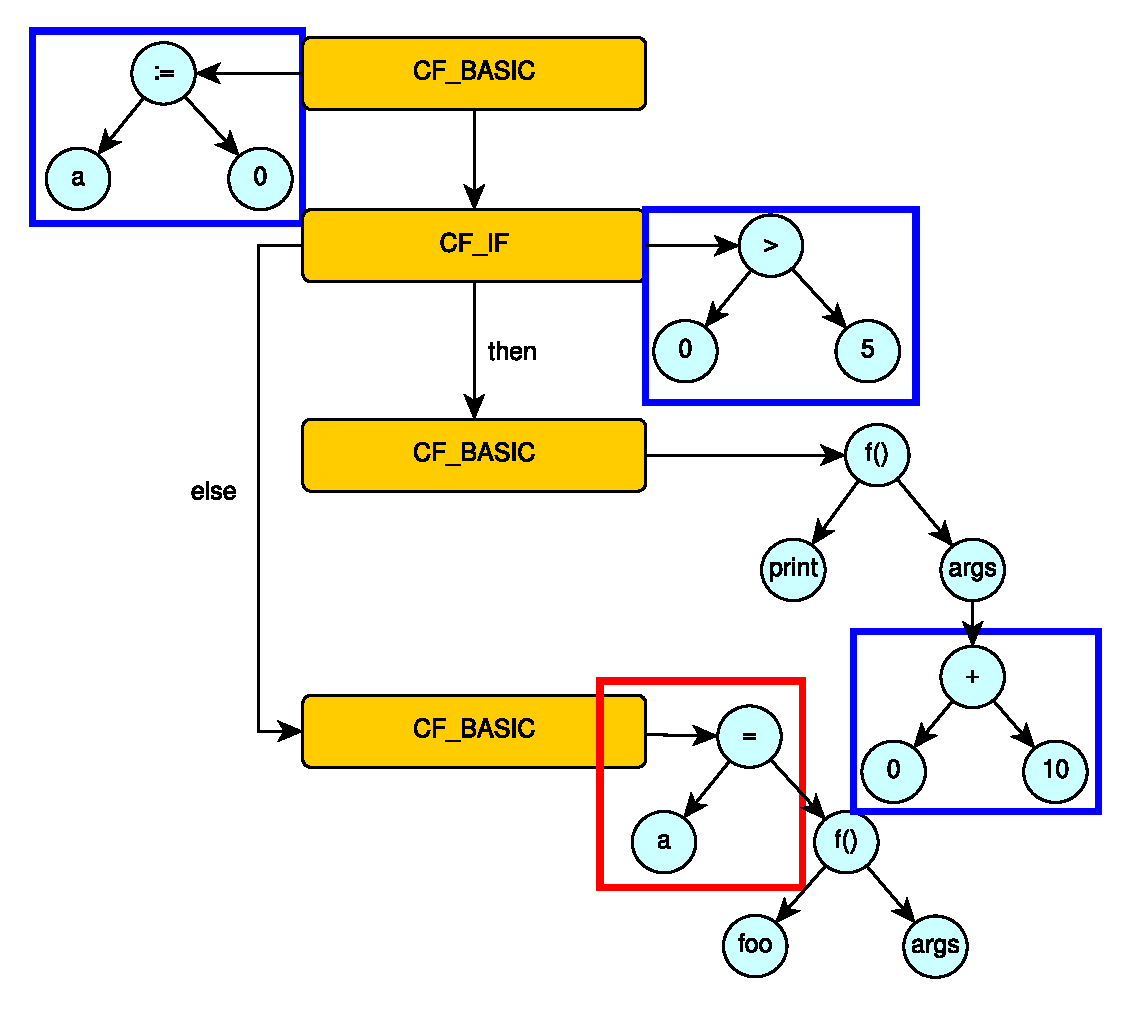
\includegraphics[height=0.8\textheight]{img/optimise1.pdf}}
    \only<3>{
    Po skládání konstant
    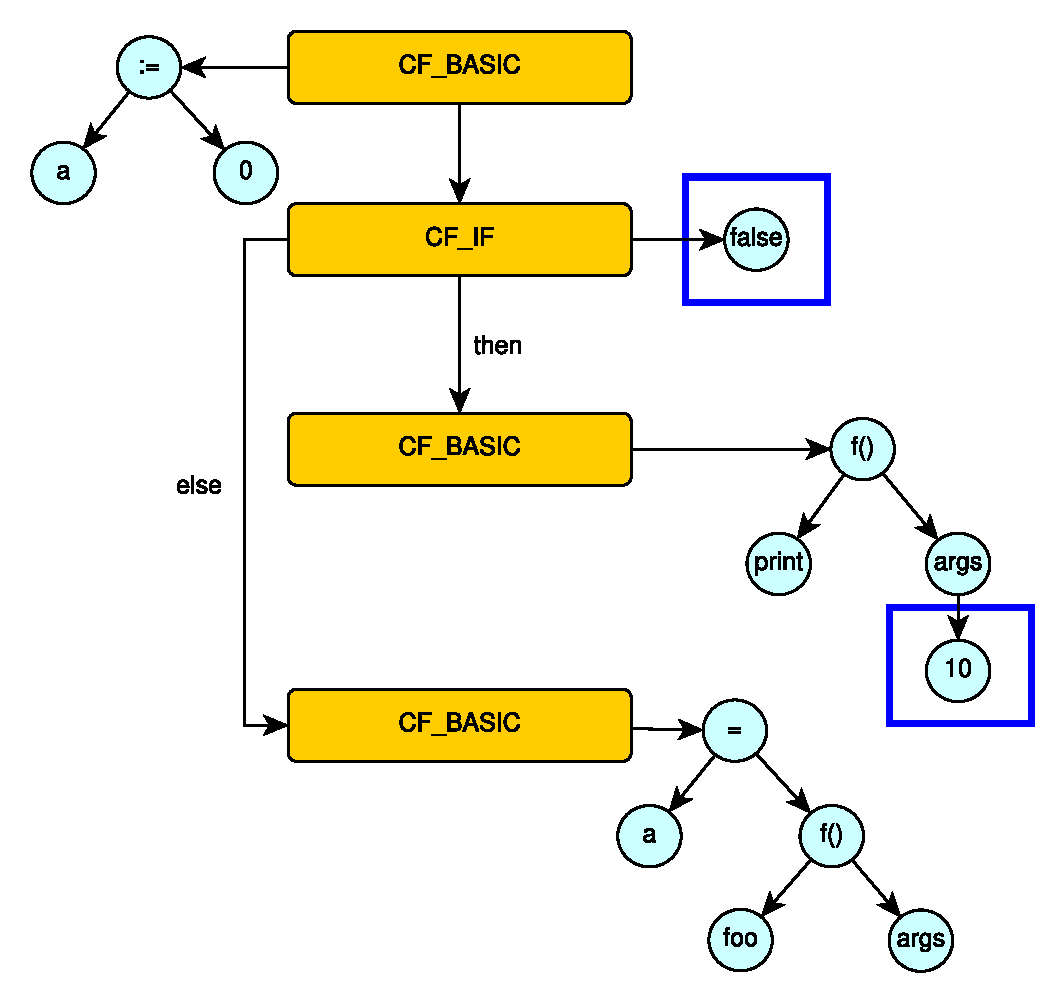
\includegraphics[height=0.8\textheight]{img/optimise2.pdf}}
    \only<4>{
    Po odstranění mrtvého kódu
    
    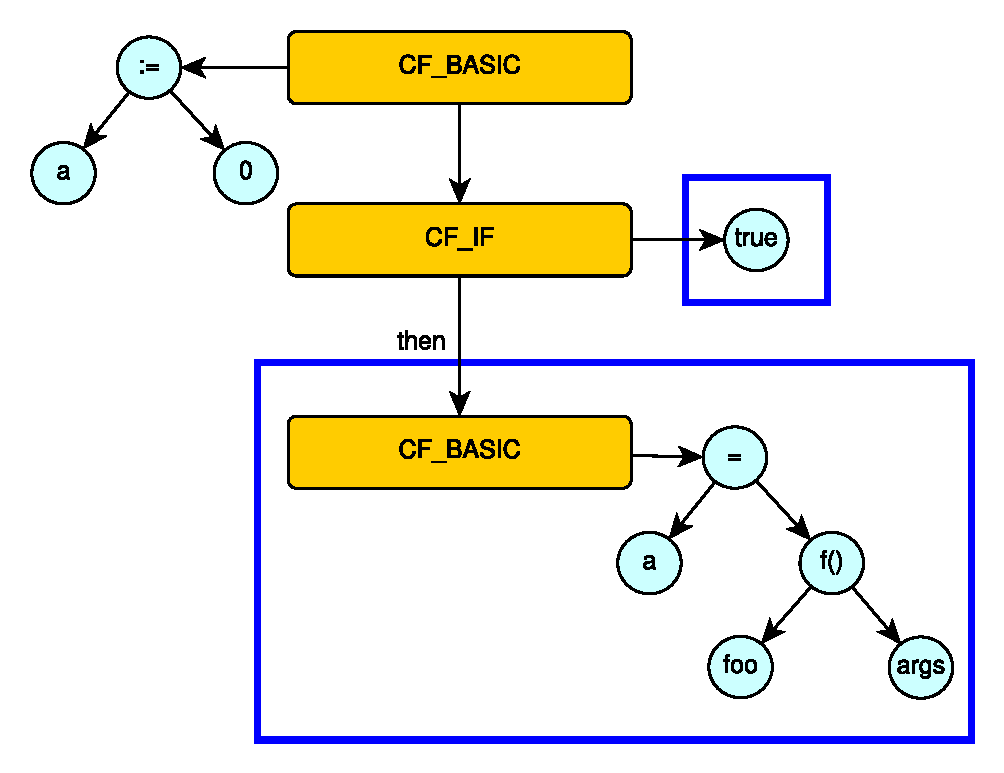
\includegraphics[height=0.8\textheight]{img/optimise3.pdf}}
\end{frame}

\begin{frame}{Generátor}
    \begin{itemize}
        \item Generování výrazů
        \begin{itemize}
            \item Post-order rekurzivní průchody jednotlivými AST
            \item Aritmetické výrazy generovány přímo na zásobníku
            \item Logické výrazy generovány zkráceným vyhodnocováním
        \end{itemize}
        \item Volání funkcí
        \begin{itemize}
            \item Argumenty v dočasném rámci, návratové hodnoty na zásobníku (integrace do vyhodnocování výrazů)
            \item Vestavěné funkce generovány \textit{in-line}
        \end{itemize}
        \item Rozsahy platnosti -- svázáno s tabulkami symbolů, dekorované názvy proměnných
        \item Dopředné generování definic proměnných
        \item Počítání referencí (zahazování zbytečných definic)
    \end{itemize}
\end{frame}

\begin{frame}{Použité datové struktury}
    \begin{itemize}
        \item Lineárně vázaný seznam (jedno- i obousměrně vázaný)
            \begin{itemize}
                \item Funkce, parametry a návratové hodnoty v~grafu řízení toku
                \item Konstanty při optimalizacích
                \item Zásobníky, tabulky symbolů
            \end{itemize}
        \item Hashovací tabulka
            \begin{itemize}
                \item Tabulka symbolů
            \end{itemize}
        \item Zásobník
            \begin{itemize}
                \item Zásobník tabulek symbolů
                \item Zásobník pro precedenční SA
            \end{itemize}
        \item Strom
            \begin{itemize}
                \item Graf řízení toku, abstraktní syntaktický strom
            \end{itemize}
        \item Nafukovací pole
        \begin{itemize}
                \item Dynamický řetězec pro načítání identifikátorů a řetězcových konstant
            \end{itemize}
    \end{itemize}
\end{frame}

\bluepage{Diskuze}

\bluepage{Děkujeme za pozornost.}

\end{document}
